% !TeX spellcheck = en_GB
\subsection{Variables and Data Transformations}
\respdist{40}{30}{30}
For this regression problem the attribute \textit{Reported thefts/burglaries per 1,000 inhabitants} (\var{RT}) has been chosen for prediction based on all features.
The goal of the regression is to predict the \var{RT} for a municipality fives years in the future. Each data point consisted of data from eight to five years prior to the year \var{RT} was predicted for, so for instance data from 2007-2010 would be used to predict \var{RT} in 2015. Only data for 2007-2018 was used, as the remaining data was not strictly comparable as explained in the previous paper, and it also has significantly more missing observations.
\\\\
Two major changes were made to the data before putting it through the models. The first was estimating missing values. This was necessary, as removing all features with even a single missing value would cause significant loss of data. Missing values were estimated by performing linear regression between the two closest values in the data sequence, which would be different observations of the same feature in different years. So for instance, $ [1, NaN, NaN, 4] $ would become $ [1, 2, 3, 4] $. This is by no means the best possible estimation, but it is good enough for our purposes considering the fairly small number of missing values (about 4\pro). If an entire sequence was missing, all values would be set to 0. The second major change was standardization, as the features varied significantly in scale. This meant subtracting the mean and dividing by the standard deviation (sd) for each feature.\\
\\
The data was shuffled and represented as a feature matrix $ \mathbf X $ and target target vector $ \mathbf y $. $ \mathbf X $ had size $ n\times D $ where $ n $ was the number of data points and $ D $ the number of features multiplied by four, as four years of data was used for each key figure. $ \mathbf y $ was an $ n $ long target vector containing the standardized \var{RT}. Finally the data was randomly split into training, validation, and test subsets.


\subsection{Regularization and Generalization Error}
\respdist{0}{100}{0}
Flexible machine learning models have a tendency to overfit.
One way to counter this is with regularization, which punishes the model for fitting weights too specifically to the data.
One would generally expect weights in a trained model to be normally distributed around zero, so weights further from zero count more towards the error.
Using L2 regularization, the term $ \lambda\len{\mathbf w}^2 $ is added to the error, where $ \lambda $ is the regularization parameter and $ \mathbf w $ a vector containing all weights, so using mean squared error loss, the error would be
\begin{equation*}
	E=\frac{1}{N}\len{\mathbf y-\hat{\mathbf y}}^2+\lambda\len{\mathbf w}^2
\end{equation*}
Performing ten-fold cross-validation with linear regression using 30 log$ _{10} $-spaced values from $ -3 $ to 3, we were able to estimate a general error by training and testing on different subsets of data and thus best estimate the optimal regularization parameter. The error can be seen on figure \ref{fig:reg}.
\begin{figure}[h!]
	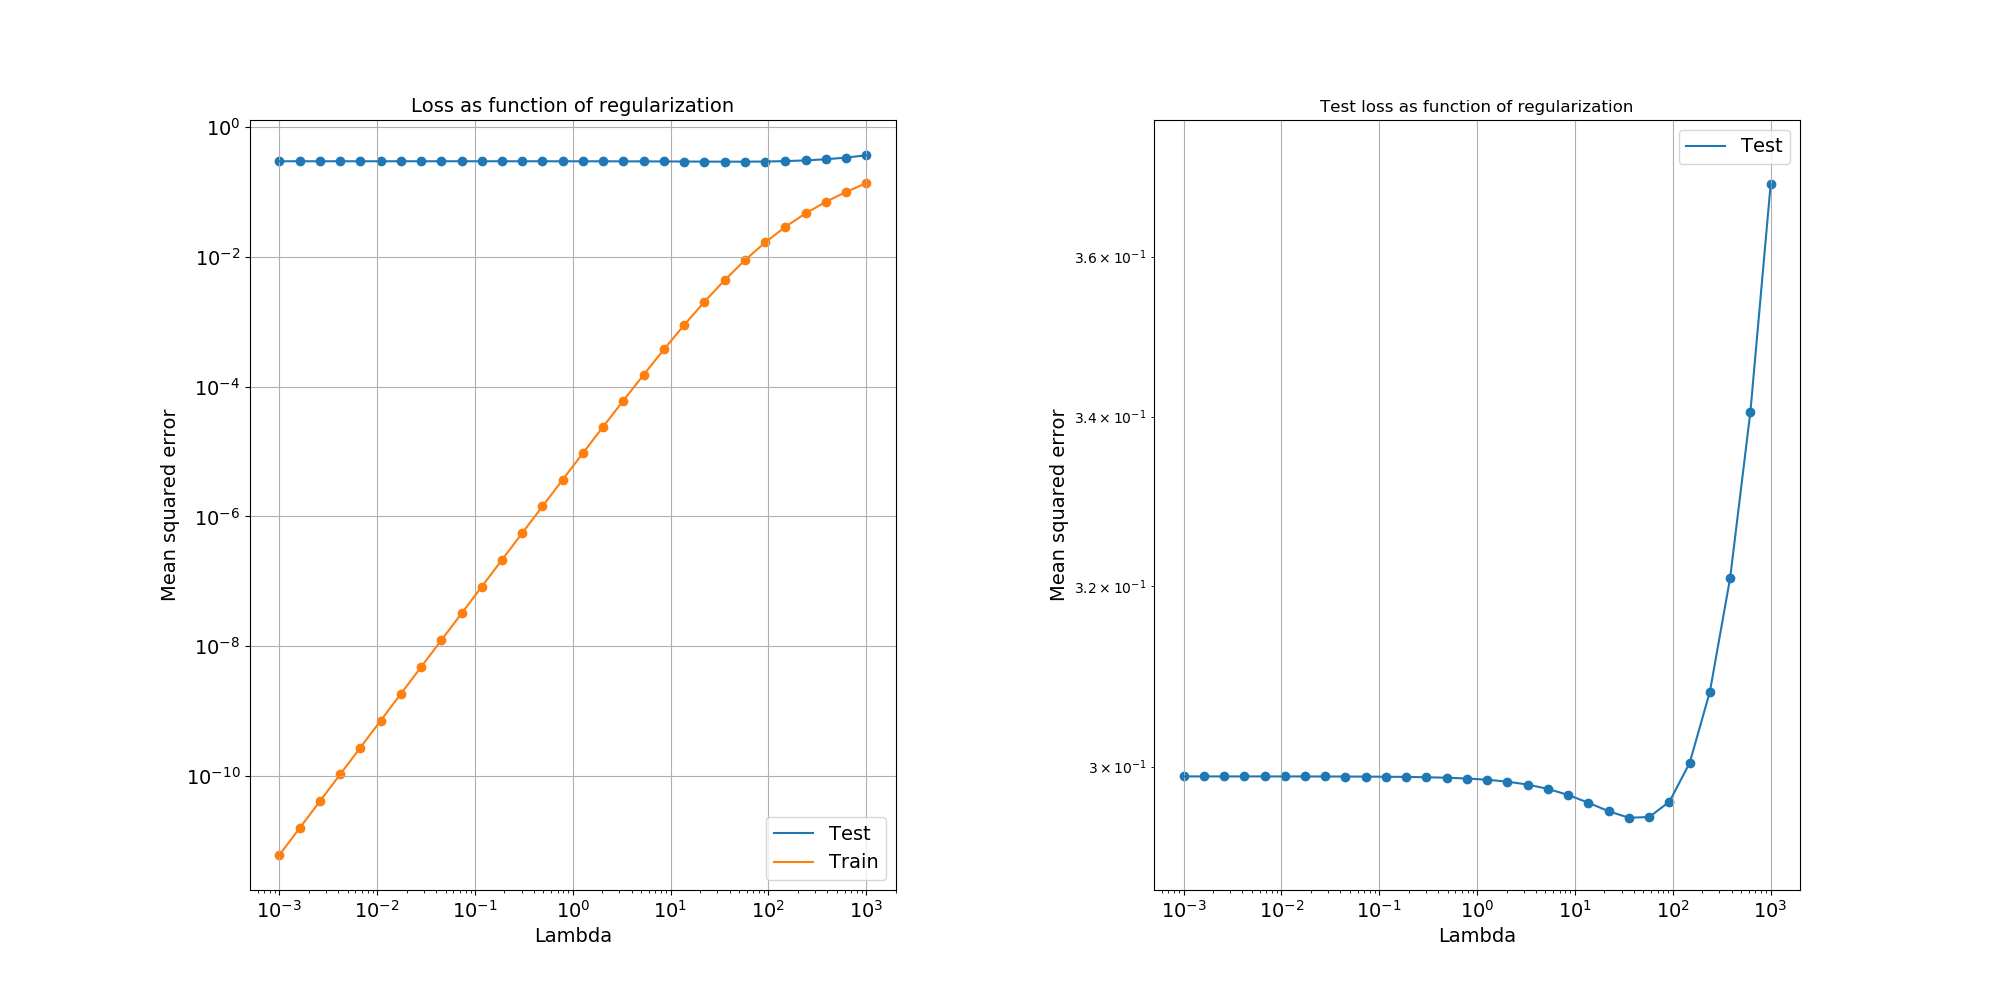
\includegraphics[width=	\textwidth]{regularization}
	\caption{Test and train loss plotted against the regularization parameters. The test loss is also shown on a separate plot, as the significant overfitting make details very hard to see.}\label{fig:reg}
\end{figure}
As expected, significant overfitting occurs for small values of $ \lambda $. It is clearly seen that an optimal value exists at roughly $ \lambda=10^{1.7} $, even if the difference is fairly small. At that point, the test loss is around 0.294, which is a slight decrease from the roughly 0.299 seen at lower values.\\
\\
To find out how the linear regression model predicts new data, the weights of the model are extracted. The 10 features with highest numerical weight value is shown in the table beneath:
\begin{table}[H]
	\centering
	\small
	\begin{tabular}{l l l}
		Order &Feature based on highest numerical weight value & Weights	\\\hline
		1-4& \textbf{RT} (1-4 years back)  		& 0.02499, 0.0248,  0.0243, 0.0228 \\
		5&"Exp. to intro. courses for foreigners per inhabitant" - three years  	& -0.01115 \\
		6-8&"Exp. to city development, housing and environment per inhabitant"\\
		& (2-4 years back) & 0.01068, 0.01058, 0.01055 \\
		9&"Exp. to intro. courses for foreigners per inhabitant" - four years  & -0.009853
		\\
		10 &"Children of single providers per 100 0-17-year-old" - 4 years back & 0.009837
	\end{tabular}
\end{table}\noindent
Is it quite natural that the \textbf{RT} feature in the previous years have the highest weights and that they appear in chronological order.
The 5th and 9th feature regards expenses to integration, which is negatively weighted, suggesting negative correlation, which makes intuitive sense.
It is not obvious why city development (feature 6-8) is positively weighted, but it may be a bad trait that high expenses are needed in relation to housing and development.
The number of children of single providers is the 10th most weighted feature, and positively so.
It noteworthy that the numerical weights of the \textbf{RT} features are more than twice as high as the next feature weight.

\subsection{Models}
\respdist{40}{60}{0}
We tested three different models for regression, described in the following parts.
In order to ensure comparability between the tests, a fixed seed was set, so the train/validation/test split and initial network parameters were all the same.


\paragraph{Baseline}
In order to have a baseline model to compare the more sophisticated models to, we implemented a simple model that would predict the mean of the training data.
The MSE for this model is $ E=\frac{1}{N}\len{\boldsymbol{\mu}_{\mathbf y}-\hat{\mathbf y}}^2 $ where $ \boldsymbol{\mu}_{\mathbf y} $ is the vector where every element is the mean of $ \mathbf y $.

\paragraph{Linear Regression}
A linear model predicts $ y $ from a linear combination of a weight vector and a feature vector, $ y=\transpose{\mathbf w}\mathbf x $.
$ w_0 $ is a bias term, and as such $ x_0 $ is always set to 1.
Organizing $ n $ data points into an $ n\times k $ feature matrix $ \hat{\mathbf X} $ and an $ n $ long vector $ \hat{\mathbf y} $, the optimal weights $ \mathbf w^* $ can be calculated by solving the matrix equation
\begin{equation*}
	(\transpose{\hat{\mathbf X}}\hat{\mathbf X}+\lambda \mathbf I)\mathbf w^*=\transpose{\hat{\mathbf X}}\hat{\mathbf{y}}
\end{equation*}
This assumes least squares optimization and L2 regularization.

\paragraph{Artificial Neural Network}
A feedforward network was implemented using the PyTorch framework.
The input layer had $ D $ neurons, and the output layer had only one neuron, as only one feature was predicted.
For the loss function, we used mean squared error loss (MSE loss) as for the other regression methods.
The network was trained using stochastic gradient descent.
All networks had a single hidden layer with a variable number of hidden neurons, $ h $, followed by the ReLU activation function.
Batch normalization and dropout was used to limit overfitting.
Based on preliminary runs, we decided to test $ 1, 2^3, 2^5, 2^7, 2^8, 2^9,\andim 2^{10} $ hidden neurons respectively.

\subsection{Two-level Cross-validation}
\respdist{80}{0}{20}
Two-level cross-validation is a method seeking to estimate the true performance of a model on data not in the dataset.
It is essentially a nested version of $ K $-fold cross-validation, and it is an effective method to compare models.
It works by first shuffling the dataset and then splitting it into $ K_1 $ training and test sets, such that every observation is in a test set exactly once.
Then for each of the training sets, the method is repeated, splitting the partition into $ K_2 $ subpartitions of training and test sets.
Every model is then trained and evaluated on these subpartitions, and the average error, $ \hat E_j^{\text{gen}} $ is estimated.
This effectively simulates training the models on different datasets and seeing how they perform under different circumstances.
For comparisons sake, we used the same partitions and subpartitions for every model and model variation.
By using the model with the lowest $ \hat E_j^{\text{gen}} $ and training and evaluating on the larger partition, we obtain the test error $ E_i^{\text{test}} $ for the best model on a given subpartition.
Finally, the overall generalization error $ \hat E^{\text{gen}} $ is estimated by averaging all $ E_i^{\text{test}} $.
We did this for the baseline model (as this has no hyperparameters, no best model was selected per partition), the linear regression model varying $ \lambda $, and the neural network varying the size of the hidden layer.
We used $ K_1=K_2=10 $. The result is show on table \ref{tab:tlcv}.
\begin{table}[H]
	\centering
	\begin{tabular}{l r r r r r}
		\jl{Outer fold}	& \multicolumn{2}{c}{ANN}	& \multicolumn{2}{c}{Linear regression}	& Baseline	\\
		\jl i&\jl{$ h_i^* $}	&\jl{$ E_i^{\text{test}} $}	&\jl{$ \lambda_i^* $}	&\jl{$ E_i^{\text{test}} $}	&\jl{$ E_i^{\text{test}} $}	\\\hline
		1&$ 2^{10} $	&1.3389	&50.87	&0.0981	&2.2400	\\
		2&$ 2^{10} $	&0.2055	&41.18	&0.0967	&0.5116	\\
		3&$ 2^{10} $	&0.5436	&62.83	&0.0951	&2.1153	\\
		4&$ 2^{10} $	&0.1019	&62.83	&0.0723	&0.5523	\\
		5&$ 2^{9} $		&0.4360	&62.83	&0.0724	&0.6550	\\
		6&$ 2^{10} $	&0.6071	&62.83	&0.0671	&1.4707	\\
		7&$ 2^{9} $		&0.3151	&62.83	&0.0577	&0.4690	\\
		8&$ 2^{9} $		&0.1576	&62.83	&0.0689	&1.2423	\\
		9&$ 2^{10} $	&0.3740	&77.61	&0.0815	&0.5119	\\
		10&$ 2^{10} $	&0.7044	&62.83	&0.0655	&0.8792 \\\hline
		\jl{$ \hat E^{\text{gen}} $}	& &0.4760	& &0.0771	& 1.0593
	\end{tabular}
	\caption{Two-level cross-validation comparing the implemented models.}\label{tab:tlcv}
\end{table}\noindent
Looking at the table, there seems to be a significant difference in performance, with linear regression being by far the best model.
While the neural network seemed to perform best with high complexity, the linear regression model performed by far the best with fairly high regularization coefficients, lowering the flexibility.
These findings will now be subjected to more rigorous statistical analysis.

\subsection{Statistical Comparision of the Three Models}
\respdist{80}{0}{20}
In order to compare the models, we used the paired $ t $-test, which allows to compare two models by their estimated generalization errors. \cite[p. 210]{bog}
For this reason, only two models are compared at any time.
This paired test determines if the difference in generalization error is statistically different from zero.
We choose a significance level $ \alpha=5\pro $.
The test is applicable, because the errors are calculated on the same $ n=K_1\cdot K_2=100 $ splits and thus are paired.
Because it cannot be assumed that the generalization errors are normally distributed, the central limit theorem is needed.
This states that a linear combination of samples from any two samples will be normally distributed for sufficiently many samples $ n $, such as the difference in generalization errors here.
The rule of thumb is at least 30 samples, which is upheld here, as $ n=100 $.
The test works by first calculating the difference in generalization errors for each partition, denoted $ \hat z $.
The lower and upper bound of the confidence interval of the difference, $ z_L\andim z_U $ respectively, are calculated using the inverse cumulative $ t $-distribution:
\begin{align}
	&z_L=\operatorname{cdf}_\tau\reci \left(\frac\alpha 2\bigg\vert \nu=n-1, \mu=\hat z, \sigma=\tilde{\sigma}\right)\label{eq:lower}\\
	&z_L=\operatorname{cdf}_\tau\reci \left(1-\frac\alpha 2\bigg\vert \nu=n-1, \mu=\hat z, \sigma=\tilde{\sigma}\right)\label{eq:upper}
\end{align}
where $ \nu $ is the degrees of freedom, and for the $ i $'th loss difference $ z_i $
\begin{equation}\label{eq:sigma}
	\tilde{\sigma}^2=\frac{1}{n(n-1)}\sum\limits_{i=1}^n(z_i-\hat z)^2
\end{equation}
The $ p $-value is then found using
\begin{equation}\label{eq:p}
	p=2\operatorname{cdf}_\tau (-\len{\hat z} \vert \nu=n-1, \mu=0, \sigma=\tilde{\sigma})
\end{equation}
The the equations \eqref{eq:lower}, \eqref{eq:upper}, \eqref{eq:sigma}, and \eqref{eq:p}, table \ref{tab:sig} was produced.
\begin{table}[H]
	\centering
	\begin{tabular}{l r r r}
		&ANN and LR	&ANN and BL&LR and BL	\\\hline
		$ \tilde{\sigma} $	&0.05147	&0.07806	&0.1157\\
		$ z_L $&$ 0.2967 $	&$ -0.7382 $	&$ -1.21179 $\\
		$ z_U $&$ 0.5010 $	&$ -0.4284 $	&$ -0.75256 $\\
		$ p $  &$ 8.2499\ctp{-12} $	&$ 3.1868\ctp{-11} $	&$ 2.1432\ctp{-13} $
	\end{tabular}
	\caption{Statistical comparison of the three different regression models.}\label{tab:sig}
\end{table}\noindent
If $ 0\notin[z_L, z_U] $, or if $ p<\alpha $ (same thing), there is a statistically significant difference in their performance.
The $ p $-value is the chance of seeing the observed value or more extreme from chance, if the null hypothesis is true -- if the true difference is 0.
As $ p $ is so small, it is extremely unlikely that there is not a significant performance difference.
We can thus conclude that both a neural network and linear regression outperform the baseline model, with linear regression being the best of the three.
Most surprising was the fact that the neural network performed relatively poorly seeing as it is a much more sophisticated model.
This could be due to overfitting, even though we tried to counter it with batch normalization, dropout, and L2 regularization, but more likely it may just not be a task well suited for a neural network.
We suspect that, as the data is sequential in nature, a recurrent neural network should perform quite well.
Using different optimizers and tuning hyperparameters could further improve performance.





















